

\chapter{Obsah elektronické přílohy}

1) Mám sem nahrát celý adresář programu? Včetně složek pro obrázky/ikony? Mám tyto složky odevzdat i s obrázky? 

2) Mám nahrát i databázové soubory .db? 

3) Mám do elektronické přilohy zařadit i dokumentaci ke krabičce nebo stačí ji zobrazit jen zde v příloze tohoto dokumentu?

musí obsahovat spustielné soubory, tedy dodat knihovny z kterých se dědí. Sice je jim to jedno, protože to není připojené ke komponentům, ale k prvnimu erroru se dostanou

\bigskip

{\small
%
\dirtree{%.
.1 /\DTcomment{kořenový adresář přiloženého archivu}.
.2 main.py.
.2 gui.py.
.2 database.py.
.2 scale.py.
.2 barcode\_sensor.py.
}
}

\bigskip
\bigskip
\bigskip

{\small
%
\dirtree{%.
.1 /\DTcomment{kořenový adresář přiloženého archivu}.
.2 firmware./\DTcomment{Složka fimwaru}.
.3 main.py.
.3 gui.py.
.3 database.py.
.3 scale.py.
.3 barcode\_sensor.py.
.3 database.db.
.3 inventory.db.
.3 Images /\DTcomment{Seznam složek obsahující obrázky}.
.4 Alcohol /\DTcomment{Obrázky destilátů}.
.4 Icons /\DTcomment{Ikony tlačítek}.
.3 lib.
.2 Barcode scaner case documentation.xx.
.2 G\&G E-3000 - Opravená verze dokumentace.pdf.
.2 ukázka funkčnosti měřicího systému.mp4.
}
}








%Elektronická příloha je často nedílnou součástí semestrální nebo závěrečné práce.
%Vkládá se do informačního systému VUT v~Brně ve vhodném formátu (ZIP, PDF\,\dots).
%
%Nezapomeňte uvést, co čtenář v~této příloze najde.
%Je vhodné okomentovat obsah každého adresáře, specifikovat, který soubor obsahuje důležitá nastavení, který soubor je určen ke spuštění, uvést nastavení kompilátoru atd.
%Také je dobře napsat, v~jaké verzi software byl kód testován (např.\ Matlab 2018b).
%Pokud bylo cílem práce vytvořit hardwarové zařízení,
%musí elektronická příloha obsahovat veškeré podklady pro výrobu (např.\ soubory s~návrhem DPS v~Eagle).
%
%Pokud je souborů hodně a jsou organizovány ve více složkách, je možné pro výpis adresářové struktury použít balíček \href{https://www.ctan.org/pkg/dirtree}{\texttt{dirtree}}.
%
%\bigskip

%{\small
%%
%\dirtree{%.
%.1 /\DTcomment{kořenový adresář přiloženého archivu}.
%.2 logo\DTcomment{loga školy a fakulty}.
%.3 BUT\_abbreviation\_color\_PANTONE\_EN.pdf.
%.3 BUT\_color\_PANTONE\_EN.pdf.
%.3 FEEC\_abbreviation\_color\_PANTONE\_EN.pdf.
%.3 FEKT\_zkratka\_barevne\_PANTONE\_CZ.pdf.
%.3 UTKO\_color\_PANTONE\_CZ.pdf.
%.3 UTKO\_color\_PANTONE\_EN.pdf.
%.3 VUT\_barevne\_PANTONE\_CZ.pdf.
%.3 VUT\_symbol\_barevne\_PANTONE\_CZ.pdf.
%.3 VUT\_zkratka\_barevne\_PANTONE\_CZ.pdf.
%.2 obrazky\DTcomment{ostatní obrázky}.
%.3 soucastky.png.
%.3 spoje.png.
%.3 ZlepseneWilsonovoZrcadloNPN.png.
%.3 ZlepseneWilsonovoZrcadloPNP.png.
%.2 pdf\DTcomment{pdf stránky generované informačním systémem}.
%.3 student-desky.pdf.
%.3 student-titulka.pdf.
%.3 student-zadani.pdf.
%.2 text\DTcomment{zdrojové textové soubory}.
%.3 literatura.tex.
%.3 prilohy.tex.
%.3 reseni.tex.
%.3 uvod.tex.
%.3 vysledky.tex.
%.3 zaver.tex.
%.3 zkratky.tex.
%%.2 navod-sablona\_FEKT.pdf\DTcomment{návod na používání šablony}.
%.2 sablona-obhaj.tex\DTcomment{hlavní soubor pro sazbu prezentace k~obhajobě}.
%%.2 readme.txt\DTcomment{soubor s~popisem obsahu CD}.
%.2 sablona-prace.tex\DTcomment{hlavní soubor pro sazbu kvalifikační práce}.
%.2 thesis.sty\DTcomment{balíček pro sazbu kvalifikačních prací}.
%}
%}

\chapter{Dokumentace krabičky čtečky čárových kódů}

V této části se nachází dokumentace a obrázky navrhnuté krabičky pro čtečku čárového kódu vytisknutou pomocí 3D tiskárny. Zasunovací víko je možné zajistit dvěma šrouby M3 délky max. 7 mm.

\begin{figure}[H]
    \begin{center}
        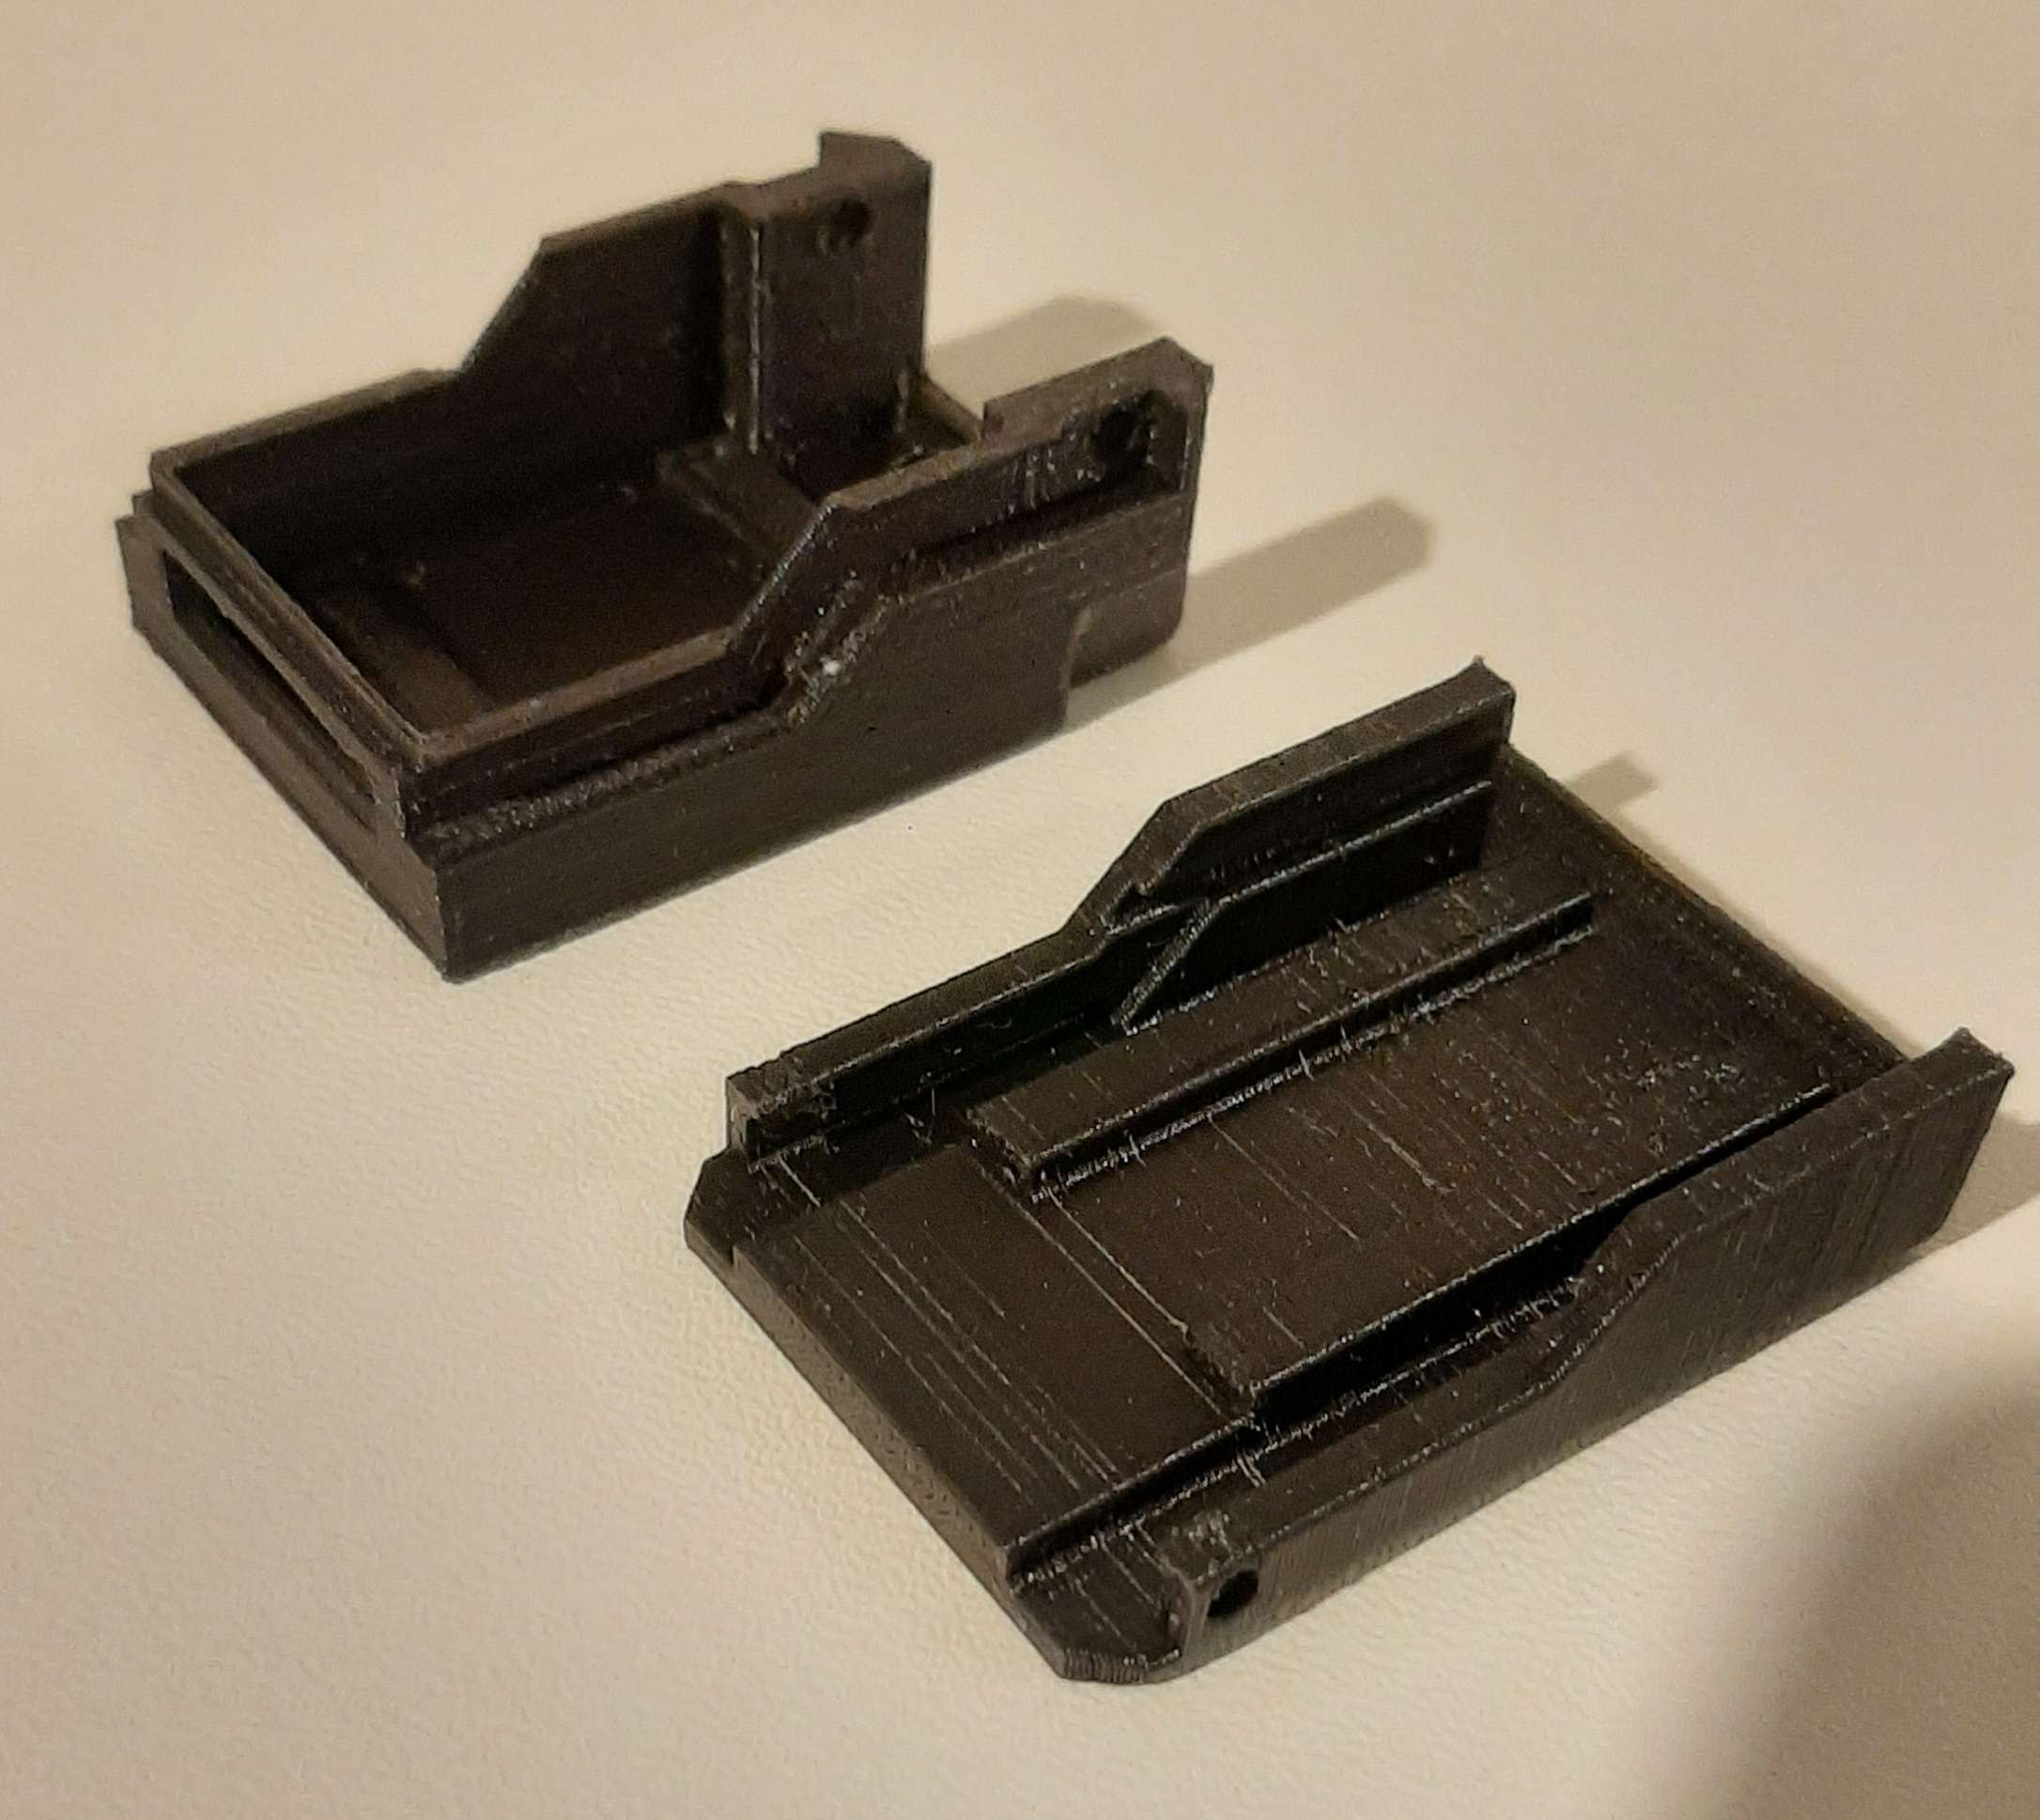
\includegraphics[scale=0.15]{obrazky/krabicka rozlozena.jpg}
    \end{center}
    \caption{Krabička čtečky čárového kódu - rozebrána}
    \label{Interakce mezi okny GUI}
\end{figure}

\begin{figure}[H]
    \begin{center}
        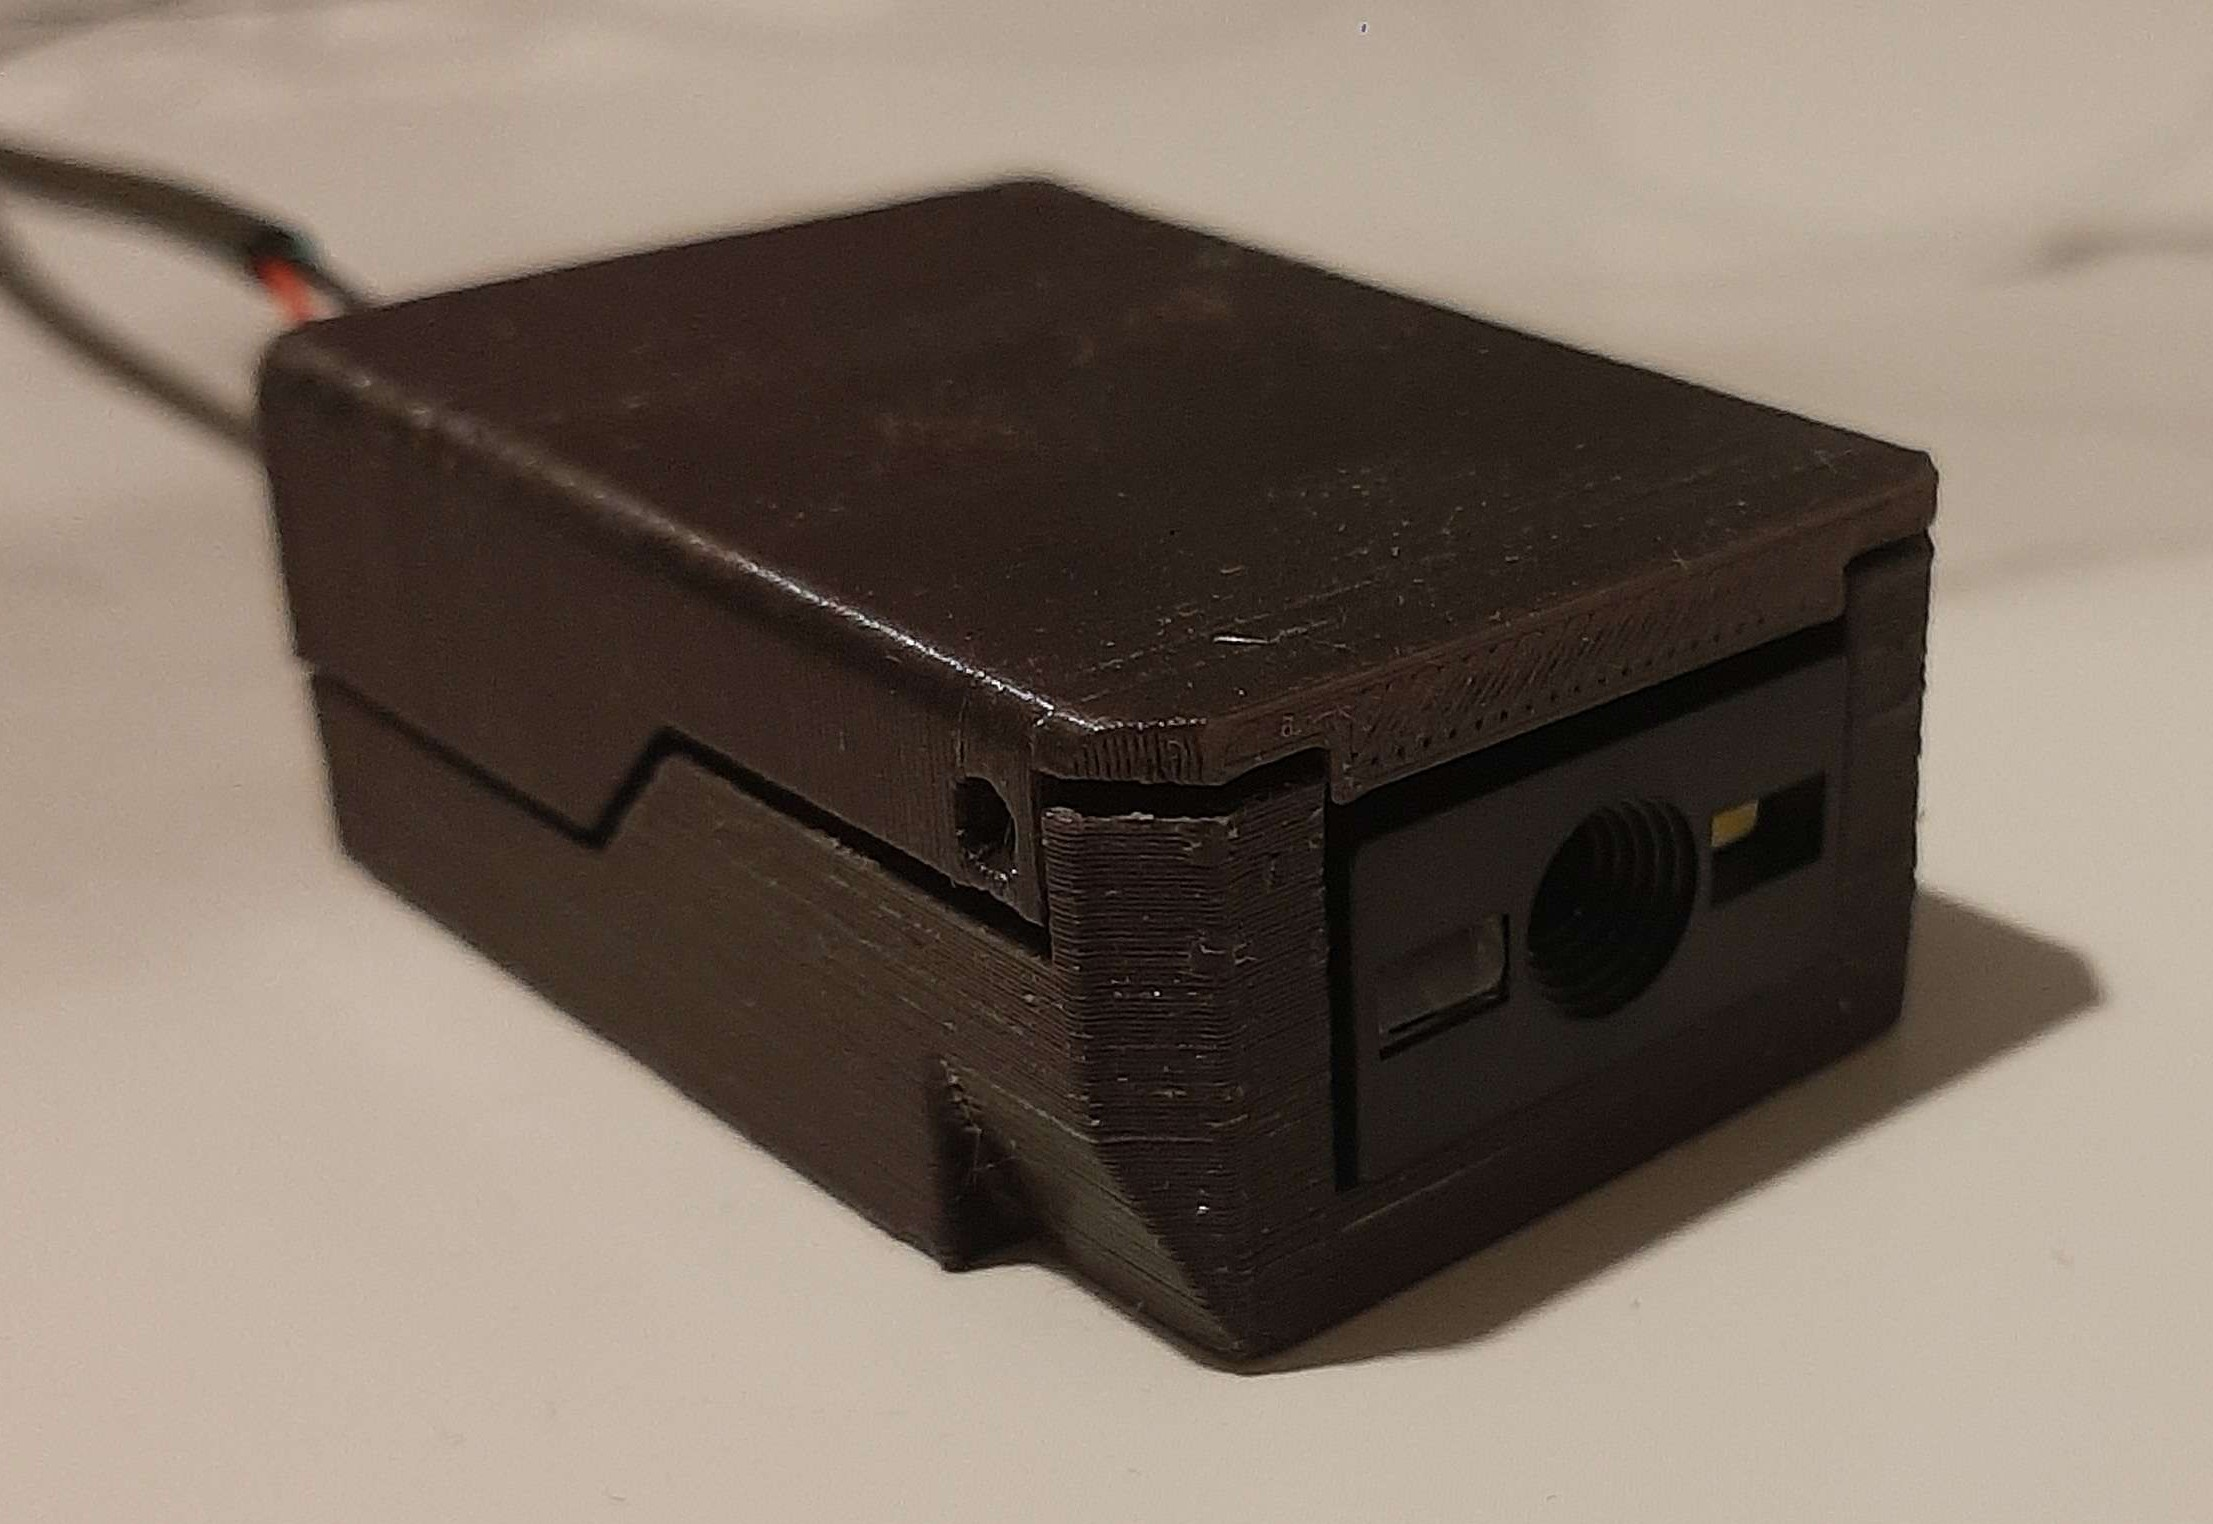
\includegraphics[scale=0.15]{obrazky/krabicka slozena.jpg}
    \end{center}
    \caption{Krabička čtečky čárového kódu - složena}
    \label{Interakce mezi okny GUI}
\end{figure}


//DODĚLAT DOKUMENTACI

\chapter{Naměřená data}

\section{Naměřené hmotnosti prázdných lahví}

\section{Tabulka naměřených objemů neotevřených lahví}

\begin{table}[h]
    \centering
    \begin{tabular}{|c|c|c|c|}
        \hline
         & \textbf{m$_{max}$ [g]} & \textbf{m$_{min}$ [g]} & \textbf{m$_{kap}$ [g]} \\ \hline \hline
        1 & 910.14 & 432.42 & 477.72 \\ \hline
        2 & 908.37 & 432.78 & 475.59 \\ \hline
        3 & 909.14 & 433.01 & 476.13 \\ \hline
        4 & 905.82 & 432.23 & 473.59 \\ \hline
        5 & 911.43 & 432.84 & 478.59 \\ \hline
        6 & 907.48 & 432.31 & 475.17 \\ \hline
        7 & 906.14 & 433.92 & 472.22 \\ \hline
        8 & 904.9 & 433.61 & 471.29 \\ \hline
        9 & 908.31 & 433.35 & 474.96 \\ \hline
        10 & 906.41 & 433.77 & 472.64 \\ \hline
        11 & 907.74 & 432.43 & 475.31 \\ \hline
        12 & 908.29 & 433.77 & 474.52 \\ \hline
        13 & 906.83 & 432.93 & 473.9 \\ \hline
        14 & 909.02 & 433.61 & 475.41 \\ \hline
        15 & 907.36 & 432.87 & 474.49 \\ \hline
    \end{tabular}
    \caption{Rozptyl hmotností plné (m$_{max}$), prázdné (m$_{min}$) láhve a jejich rozdíl (m$_{kap}$) - Amundsen vodka 0,5 l}
    \label{tab:placeholder_label}
\end{table}


\section{Průběhy, výpočty a tabulky nárůstu hmotnosti z důvodu orosení}

\begin{equation}
T_{ds} = \frac{243,5 \cdot ln(\frac{V}{100} \cdot e^{\frac{17,67 \cdot T}{243,5 + T}})}{17,67 - ln(\frac{V}{100} \cdot e^{\frac{17,67 \cdot T}{243,5 + T}})}
\label{rosný bod obecne}
\end{equation}
%\caption{Rovnice rosného bodu}

\(T_{ds}\) ...Rosný bod \([\mathrm{^\circ C}]\)

\(V\) ...Relativní vlhkost vzduchu \([\mathrm{\%}]\)

\(T\) ...Teplota vzduchu \([\mathrm{^\circ C}]\)

\begin{equation}
T_{ds} = \frac{243,5 \cdot ln(\frac{50}{100} \cdot e^{\frac{17,67 \cdot 20}{243,5 + 20}})}{17,67 - ln(\frac{50}{100} \cdot e^{\frac{17,67 \cdot 20}{243,5 + 20}})} = 9,27 [^\circ C]
\label{rosný bod}
\end{equation}
%\caption{Požadavek na orosení T\_ds> 5 °C}

\bigskip

% Requires: \usepackage{graphicx}
\begin{table}[H]
    \centering
    \begin{tabular}{|c|c|c|c||c|c|c|}
    \hline
    \begin{tabular}[c]{@{}c@{}}čas \\ ´[min]\end{tabular} & 
    \begin{tabular}[c]{@{}c@{}}Božkov vaj. \\ lik. (0,5 l) [g]\end{tabular} & 
    \begin{tabular}[c]{@{}c@{}}Heffron \\ (0,7 l) [g]\end{tabular} & \begin{tabular}[c]{@{}c@{}}Nivnice \\ bor. (1 l) [g]\end{tabular} & 
    \begin{tabular}[c]{@{}c@{}}$\Delta$m \\ Božkov [g]\end{tabular} & \begin{tabular}[c]{@{}c@{}}$\Delta$m \\ Heffron [g]\end{tabular} & \begin{tabular}[c]{@{}c@{}}$\Delta$m \\ Nivnice [g]\end{tabular} \\ \hline \hline
    0  & 846.02 & 1190.02 & 1487.09 & 0.00 & 0.00 & 0.00 \\ \hline
    1  & 846.06 & 1190.03 & 1487.16 & 0.04 & 0.01 & 0.07 \\ \hline
    2  & 846.09 & 1190.05 & 1487.16 & 0.07 & 0.03 & 0.07 \\ \hline
    3  & 846.09 & 1190.09 & 1487.12 & 0.07 & 0.07 & 0.03 \\ \hline
    4  & 846.12 & 1190.09 & 1487.16 & 0.10 & 0.07 & 0.07 \\ \hline
    5  & 846.15 & 1190.12 & 1487.22 & 0.13 & 0.10 & 0.13 \\ \hline
    6  & 846.12 & 1190.22 & 1487.36 & 0.10 & 0.20 & 0.27 \\ \hline
    7  & 846.14 & 1190.21 & 1487.36 & 0.12 & 0.19 & 0.27 \\ \hline
    8  & 846.18 & 1190.22 & 1487.39 & 0.16 & 0.20 & 0.30 \\ \hline
    9  & 846.14 & 1190.25 & 1487.45 & 0.12 & 0.23 & 0.36 \\ \hline
    10 & 846.18 & 1190.31 & 1487.52 & 0.16 & 0.29 & 0.43 \\ \hline
    15 & 846.19 & 1190.32 & 1487.56 & 0.17 & 0.30 & 0.47 \\ \hline
    20 & 846.13 & 1190.35 & 1487.53 & 0.11 & 0.33 & 0.44 \\ \hline
    25 & 846.14 & 1190.31 & 1487.57 & 0.12 & 0.29 & 0.48 \\ \hline
    30 & 846.14 & 1190.37 & 1487.62 & 0.12 & 0.35 & 0.53 \\ \hline
    35 & 846.13 & 1190.38 & 1487.62 & 0.11 & 0.36 & 0.53 \\ \hline
    40 & 846.19 & 1190.47 & 1487.69 & 0.17 & 0.45 & 0.60 \\ \hline
    45 & 846.17 & 1190.41 & 1487.71 & 0.15 & 0.39 & 0.62 \\ \hline
    50 & 846.13 & 1190.46 & 1487.74 & 0.11 & 0.44 & 0.65 \\ \hline
    55 & 846.12 & 1190.39 & 1487.68 & 0.10 & 0.37 & 0.59 \\ \hline
    60 & 846.12 & 1190.30 & 1487.67 & 0.10 & 0.28 & 0.58 \\ \hline
    \end{tabular}
    \caption{Vliv orosení na hmotnost láhve}
    \label{tab:measurement_data}
\end{table}

\begin{figure}[H]
    \begin{center}
        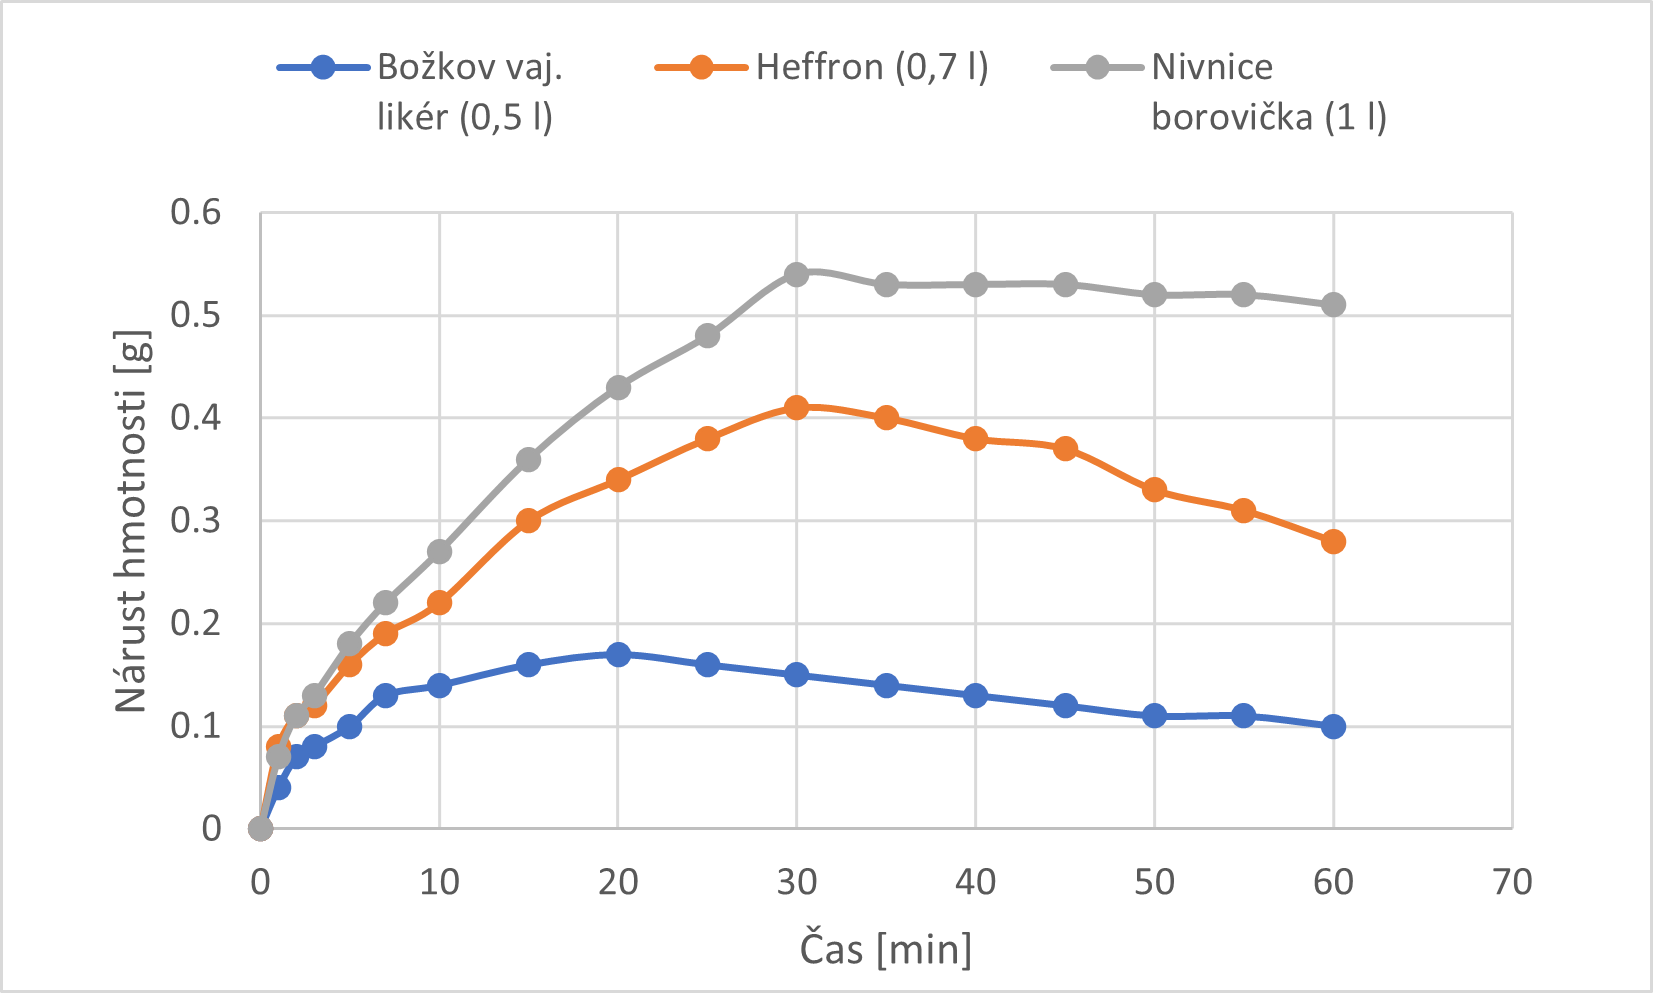
\includegraphics[scale=1.2]{obrazky/orosení.png}
    \end{center}
    \caption{Nárůst hmotnosti při orosení láhve}
\end{figure}

\chapter{Ostatní okna grafického prostředí firemwaru}

\begin{figure}[!h]
    \begin{center}
        
\includegraphics[scale=0.22]{obrazky/GUI Spuštění inventury.png}
        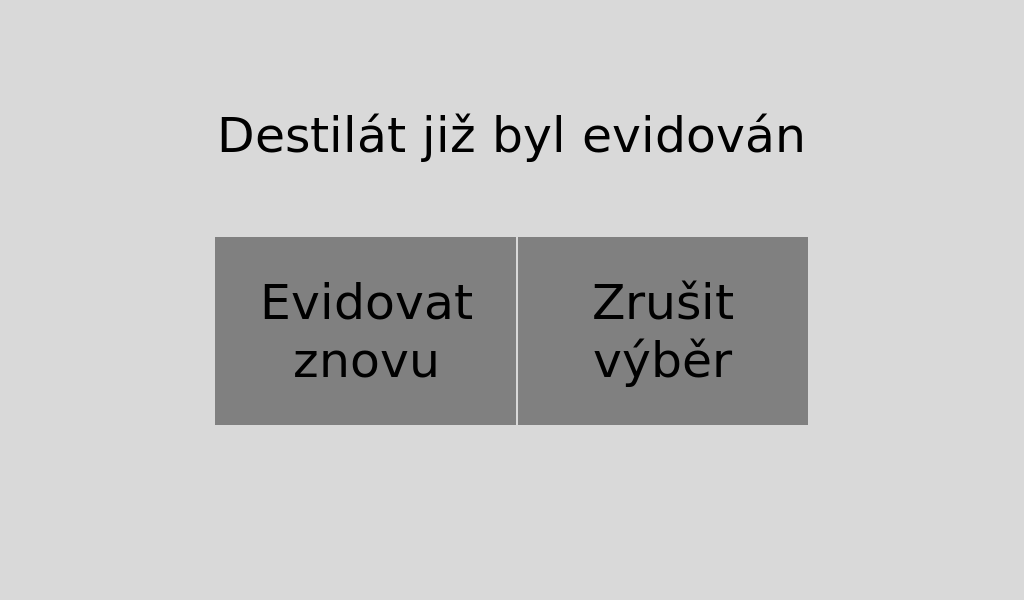
\includegraphics[scale=0.22]{obrazky/GUI Duplicidita.png}  
    \end{center}
    \caption{Úvodní okno firemwaru}
    \label{Úvodní okno aplikace}
\end{figure}

%\begin{figure}[H]
%    \begin{center}
%        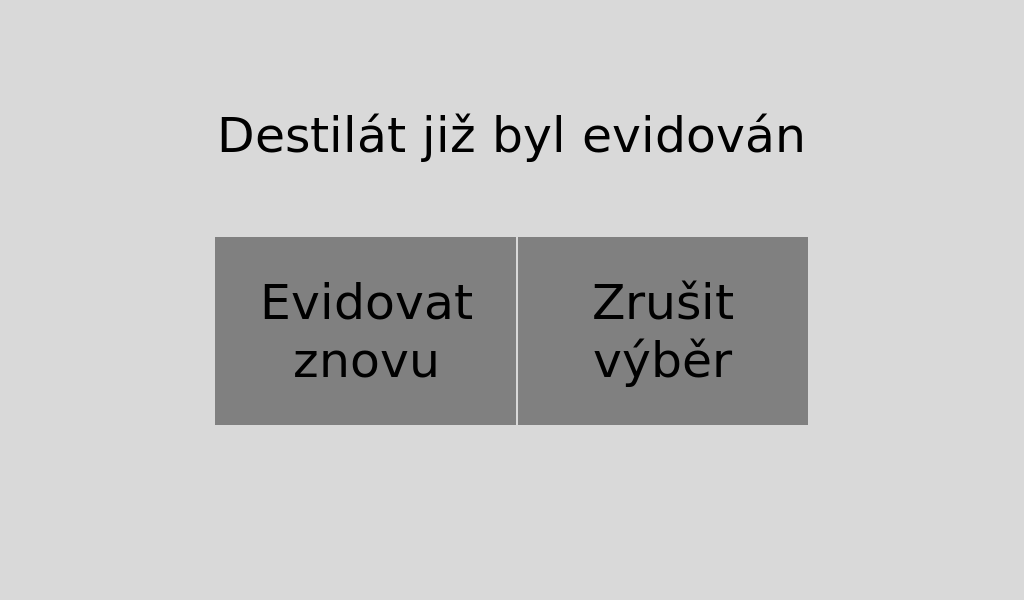
\includegraphics[scale=0.4]{obrazky/GUI Duplicidita.png}
%    \end{center}
%    \caption{Okno informující o duplicitní evidenci produktu}
%    \label{Okno informující o duplicitní evidenci produktu}
%\end{figure}

\begin{figure}[H]
    \begin{center}
        \includegraphics[scale=0.2]{obrazky/GUI Nastavení.png}
        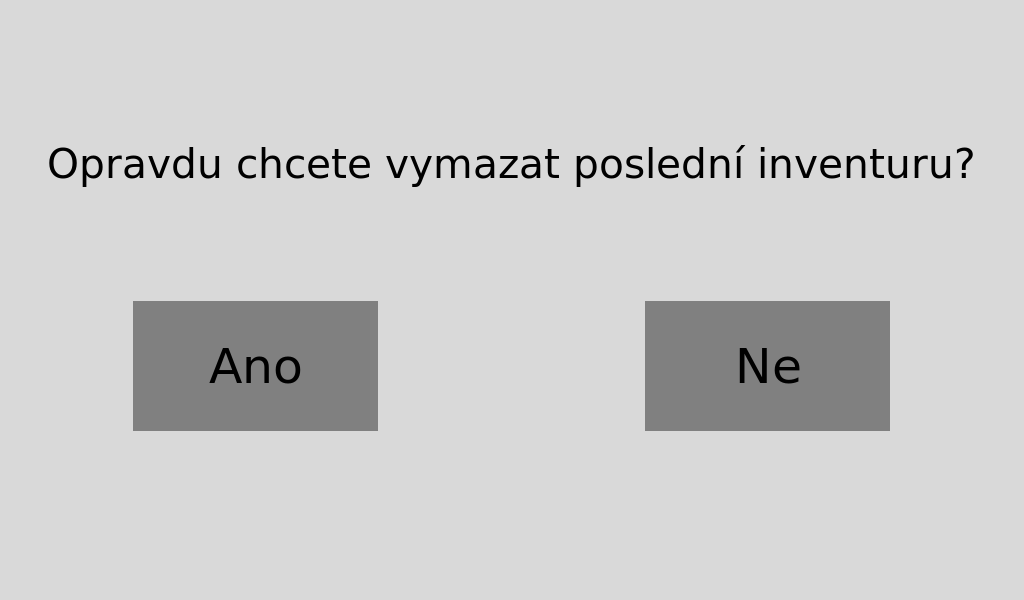
\includegraphics[scale=0.2]{obrazky/GUI Vymazání inventury.png}
    \end{center}
    \caption{Okno s nastavením firemwaru}
    \label{Okno s nastavením aplikace}
\end{figure}

\begin{figure}[H]
    \begin{center}
        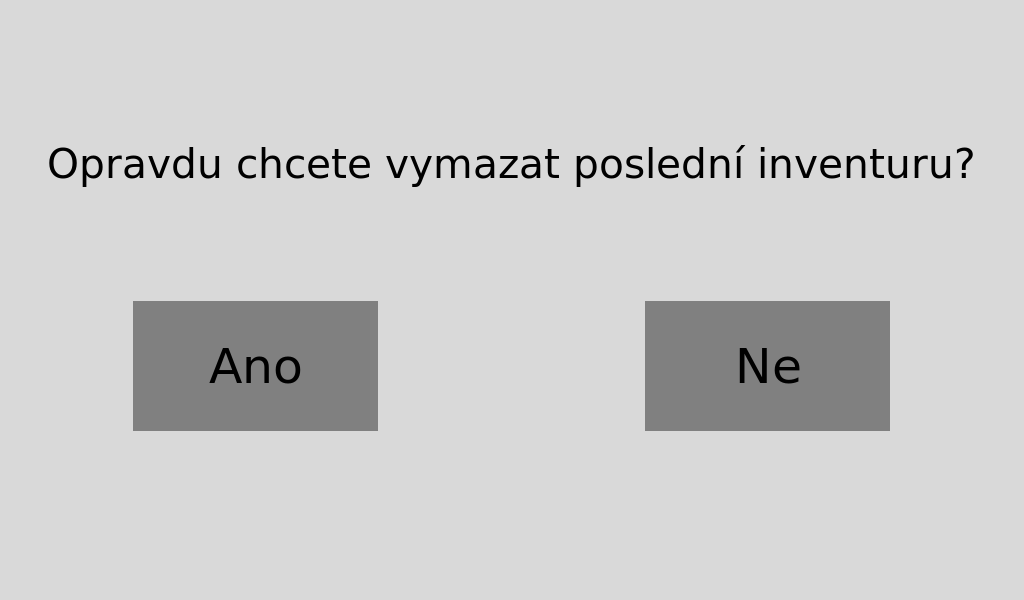
\includegraphics[scale=0.4]{obrazky/GUI Vymazání inventury.png}
    \end{center}
    \caption{Potvrzovací okno pro vymazání aktuálně spuštěné inventury}
    \label{Potvrzovací okno pro vymazání aktuálně spuštěné inventury}
\end{figure}



\chapter{Příručka GUI}
